\chapter{Validating Plate Boundary Observatory borehole
strainmeter data with GNSS derived strain}

\section{Introduction}
The Plate Boundary Observatory (PBO) contains 82 borehole strain
meters (BSMs), most of which are installed along the western United
States. BSMs are able to detect geophysical processes such as
coseismic and postseismic deformation
\citep[e.g.,][]{Langbein2006,Langbein2015}, slow slip events (SSEs)
\citep[e.g.,][]{Dragert2011}, and seismic wave propagation
\citep{Barbour2017}. BSMs are intended for measuring deformation over
timescales of minutes to months. At longer timescales, BSM data is
contaminated by factors such as borehole relaxation
\citep{Gladwin1987}. SSEs and postseismic deformation occur on
timescales that near the upper limit of what BSMs can be expected to
resolve. Another complication with BSM data is that the strain
measured at the borehole may deviate from the regional strain due to
local topographic or geologic features \citep{Berger1976}. Due to
these sources of noise, it can be difficult to use BSM data
quantitatively in, for example, geophysical inverse problems. In this
study, we assess the ability of BSMs to measure strain resulting from
SSEs on the Cascadia subduction zone. This is done by comparing BSM
data to strain derived from GNSS data.

\begin{figure}
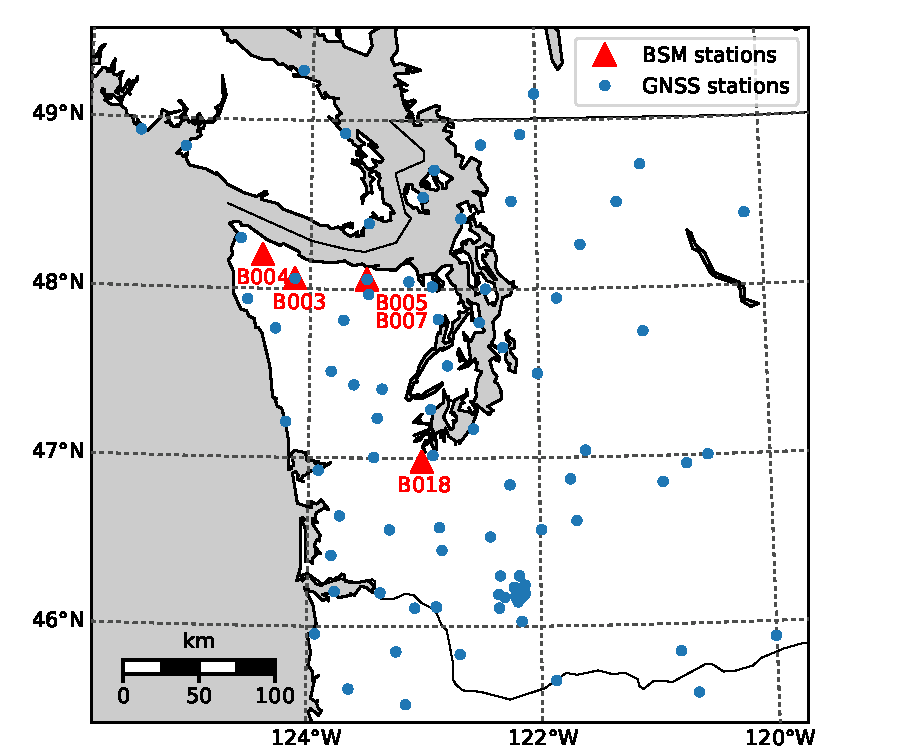
\includegraphics{ch6/figures/map.pdf}
\caption
[Location of BSM and GNSS stations used in this study]
{Location of BSM and GNSS stations used in this study.}   
\label{ch6:fig:Map}
\end{figure}

\section{BSM Data}
The are about forty PBO BSMs in the Pacific Northwest, and only five
of them, B003, B004, B005, B007, and B018, record noticeable
deformation from SSEs. We limit our attention to these five station in
this study.  The remaining stations either contain too much noise on
the timescale of SSEs or are too far away from the SSEs to observe any
strain. Each of the PBO BSMs are Gladwin four-component tensor
strainmeters, which are about 2 m long, 8.7 cm in diameter, and are
installed at about 100 to 200 m depth. Each BSM contains four
extensometers, or gauges. Only three gauges are necessary to
completely determine the horizontal strain tensor, and the fourth
gauge is included for redundancy. Gauges 1, 2, and 3 are oriented
$60^\circ$, $120^\circ$, and $150^\circ$ counterclockwise from gauge
0.

We use the level 2 gauge data provided by UNAVCO at www.unavco.org,
which has undergone several post-processing steps. In the level 2
gauge data a borehole curing trend is estimated and removed by fitting
two exponential terms and a linear trend to the data. The level 2 data
is corrected for tidal strains by estimating and removing sinusoids
with known tidal frequencies. There is also a correction for
barometric pressure because the normal stress imposed on the surface
by barometric pressure results in horizontal strains recorded by the
BSM. The barometric pressure correction is the observed barometric
pressure at each site multiplied by a best fitting scaling factor.
Lastly, offsets have been removed in the level 2 data product.

We denote the extension measured at gauge $i$ as $e_i$, and the
horizontal strain tensor components as $\varepsilon_{xx}$,
$\varepsilon_{yy}$, and $\varepsilon_{xy}$, where $x$ and $y$ indicate
the east and north direction, respectively. The extensions measured at
BSMs are traditionally converted to areal strain, $\varepsilon_a =
\varepsilon_{xx} + \varepsilon_{yy}$, differential strain,
$\varepsilon_d = \varepsilon_{xx} - \varepsilon_{yy}$, and engineering
shear strain, $\varepsilon_s = 2\varepsilon_{xy}$. We follow this
convention and use $\varepsilon_a$, $\varepsilon_d$, and
$\varepsilon_s$ for comparing BSM data to GNSS derived strains. Using
$\theta_0$ to denote the orientation of gauge 0, in degrees north of
east, these strain components can be expressed in terms of the gauge
measurements through the equation
\begin{equation}\label{ch6:eq:GaugeToStrain}
\left[\begin{array}{c}
\varepsilon_a \\
\varepsilon_d \\
\varepsilon_s \\
\end{array}\right]
=
2\mathbf{K}^{-1}\left[\begin{array}{ccc}
1 & \cos(2\theta_0) & \sin(2\theta_0) \\
1 & \cos(2(\theta_0 + 60)) & \sin(2(\theta_0 + 60)) \\
1 & \cos(2(\theta_0 + 120)) & \sin(2(\theta_0 + 120)) \\
1 & \cos(2(\theta_0 + 150)) & \sin(2(\theta_0 + 150)) \\
\end{array}\right]^+
\left[\begin{array}{c}
e_0 \\
e_1 \\
e_2 \\
e_3 \\
\end{array}\right],
\end{equation} 
where ``$+$" indicates the Moore-Penrose pseudoinverse and
$\mathbf{K}$ is a coupling matrix describing how the instrument
strains relate to the crustal strains \citep{Hart1996}. The components
$\varepsilon_a$, $\varepsilon_d$, and $\varepsilon_s$ represent
crustal strains, and $e_i$ are instrument strains. We assume that BSMs
are installed in homogeneous, isotropic rock, allowing us to write the
coupling matrix as
\begin{equation}\label{ch6:eq:CouplingMatrix}
\mathbf{K} = 
\left[\begin{array}{ccc}
c & 0 & 0 \\
0 & d & 0 \\
0 & 0 & d \\
\end{array}\right],
\end{equation}  
where $c$, and $d$ are response factors that depend on the elastic
properties of the instrument, the grout, and surrounding rock
\citep{Gladwin1985}. Based on the analysis of \citet{Gladwin1985}, we
use $c=1.5$ and $d=3.0$. UNAVCO, the organization responsible for
maintaining the PBO BSMs and disseminating their data, use these same
response factors for their final data products.

Local topographic or geologic features can cause $\mathbf{K}$ to have
non-zero off diagonal elements. If possible, the components of
$\mathbf{K}$ should be determined in-situ by calibrating the BSM data
with a well known strain source, such as diurnal and semi-diurnal
tides \citep{Hart1996,Roeloffs2010,Hodgkinson2013}. \citet{Hart1996}
calibrated a BSM at Pinyon Flat, using the tidal strains recorded at a
collocated laser strain meter. This calibration method is, of course,
not possible for most PBO BSMs. \citet{Roeloffs2010} and
\citet{Hodgkinson2013} calibrated PBO BSMs using theoretical
predictions of tidal strains \citep[e.g.,][]{Agnew1997}. This approach
is still not adequate for BSMs near large local bodies of water, which
can make it difficult to form an accurate theoretical estimate of
tidal strains. As determined by \citet{Roeloffs2010}, the five BSM
stations considered in this paper are too close to the Straight of
Juan de Fuca to be accurately calibrated with tidal strains. Since
in-situ calibration is not possible, we note that our choice for
$\mathbf{K}$ is likely to be a significant source of error in BSM
data. Another potential source of error is the assumed orientation for
$\theta_0$. This orientation is determined by a compass on the
instrument, and it is possible that magnetic minerals in the
surrounding rock can give the compass an incorrect reading.

\section{GNSS derived strain}
We compare the BSM strain components to transient strains estimated
from GNSS data. Here we consider transient strains to be any deviation
from the secular strain rate.  We use daily GNSS displacement
solutions for 94 continuous GNSS stations in the Pacific Northwest
(Figure \ref{ch6:fig:Map}). This data has also been made available through
UNAVCO. We convert the GNSS data to transient strains using Gaussian
process regression (GPR) as described in \citet{Hines2017a}. With GPR,
we select a prior spatio-temporal covariance model for the geophysical
signal that we want to recover. Following \citet{Hines2017a}, we
assume that our prior for displacements is a Gaussian process with
zero mean, and covariance function described by
\begin{equation}\label{cov}
C_u((t,x),(t',x')) = \phi^2 T(t,t')X(x,x'),
\end{equation}        
where $T$ is the Wendland covariance function
\begin{equation}\label{ch6:eq:Wendland}
T(t,t') = \left(1 - \frac{|t - t'|}{\tau}\right)^5_+ \left(\frac{8|t - t'|^2}{\tau^2} + \frac{5|t - t'|}{\tau} + 1\right), 
\end{equation}
and $X$ is the squared exponential covariance function
\begin{equation}\label{ch6:eq:SE}
X(\vec{x},\vec{x}') = \exp\left(\frac{-||\vec{x} - \vec{x}'||_2^2}{2 \ell^2}\right).
\end{equation}
The hyperparameters $\phi$, $\tau$, and $\ell$ control the amplitude,
characteristic time-scale, and characteristic length-scale of the
prior, respectively. \citet{Hines2017a} found that the optimal
hyperparameters for describing displacements from SSEs are roughly
$\phi =$ 0.5 mm, $\tau =$ 0.1 yr, and $\ell =$ 100 km. These
parameters were chosen objectively using maximum likelihood methods;
however based on our experience, this prior may not be sufficiently
flexible to described all the observed data. Consequently, we explore
using lower values for $\tau$ and $\ell$ and a higher value for
$\phi$. For each tested set of hyperparameters, we condition the prior
with the observed GNSS data and visually compare the posterior
displacements to the observations. We settle on the values $\phi =
1.0$ mm, $\tau =$ 0.05 yr, and $\ell =$ 80 km. With this final set of
hyperparameters, we condition the prior with the GNSS data and then
spatially differentiate the posterior displacements to obtain
transient strain.

\begin{figure}
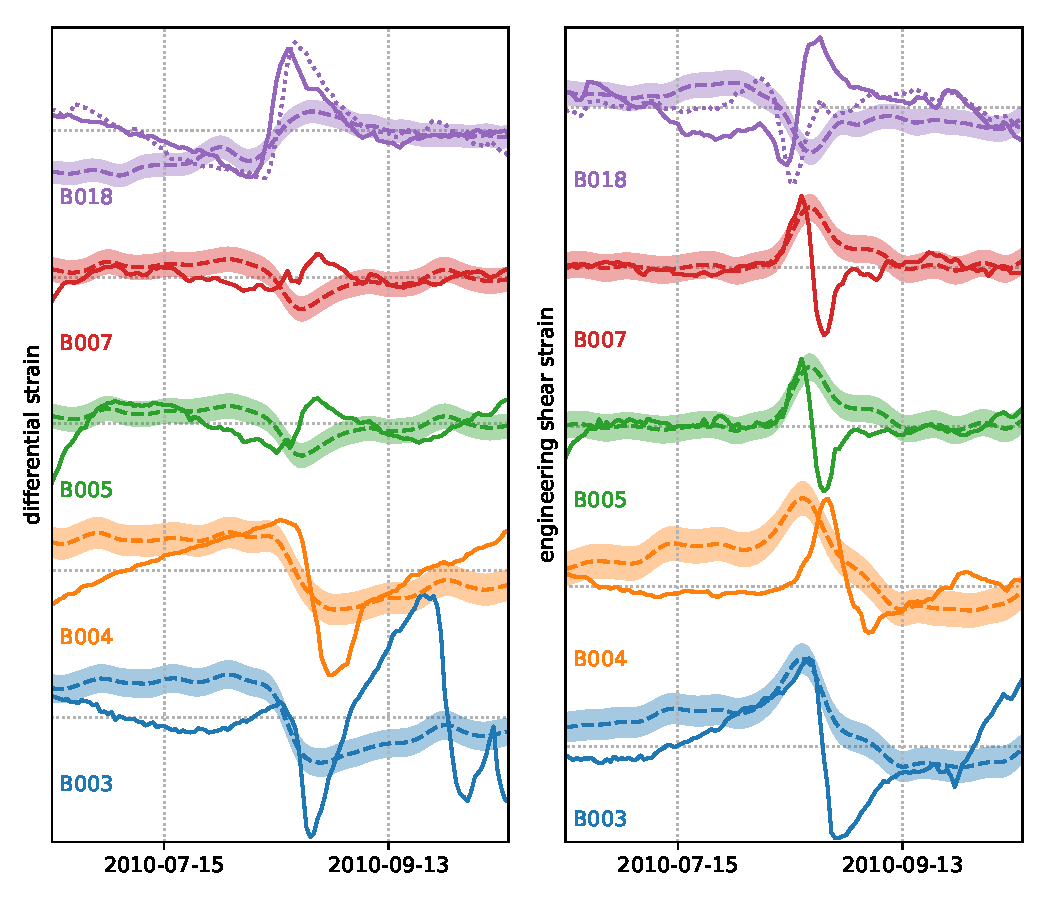
\includegraphics{ch6/figures/SSE1.pdf}
\caption
[BSM and GNSS derived strains for the summer 2010 SSE]
{differential (left) and engineering shear (right) strains
during the summer 2010 SSE observed at BSMs (solid) and derived from
GNSS data (dashed). The horizontal dotted lines are spaced by 0.1
micro-strain. The shaded region around the GNSS derived strains show
the one standard deviation confidence interval. The dotted line for
station B018 shows the BSM data using the optimal instrument
orientation. The shown BSM data has been detrended by estimating and
removing a second-order polynomial from each timeseries.}
\label{ch6:fig:SSE1}
\end{figure}

\section{Results}
We compare the BSM data to GNSS derived strains for eight SSEs in the
Puget Sound region. The earliest SSE considered occurred in spring
2009 and the latest SSE occurred in winter 2017. The two datasets are
in best agreement for the summer 2010 SSE, which is shown in Figure
\ref{ch6:fig:SSE1}. The data for the remaining SSEs are included at the
end of this manuscript in Figures \ref{ch6:fig:SSE0} through
\ref{ch6:fig:SSE7}. We only show the differential and engineering shear
strains because there is no clear signal in the areal strain for
either the GNSS derived strains or the BSM data. \citet{Roeloffs2010}
also expressed doubt in the areal strains measured at stations B003,
B004, B007, and B018 because the areal strains derived from different
combinations of gauges at these stations are not self consistent.
\citet{Roeloffs2010} also noted an inconsistency in the differential
strains at B003.

Station B004 records differential and engineering shear strains that
are most consistent with the GNSS derived strains. However, the
initiation of SSE strains recorded at B004 tend to lag several days
behind the GNSS derived strains. The strain rates recorded at B004
also tend to be greater than the GNSS derived strains. One possible
explanation for this discrepancy is that the GNSS station spacing is
too wide to resolve a relatively sharp pulse of strain from the SSE as
it traverses along the subduction zone.

The engineering shear strain, but not the differential strain,
recorded at B003 contain a clear signal from each SSE that is
consistent with the GNSS derived strains. Similar to B004, the
recorded strain rates exceed those predicted by the GNSS data. There
are many spurious features in the differential strains recorded at
B003, which makes it difficult determine whether or not that component
contains signal from SSEs.

Stations B005 and B007, which are located within a few hundred meters
of each other, both show clear SSE signals in their engineering shear
strains.  However, the temporal pattern of strain recorded at these
stations are not consistent with the GNSS derived strains.  For the
summer 2010 and summer 2011 SSEs, the GNSS derived strains predict a
single positive pulse of engineering shear strain at these locations,
but both B005 and B007 record an initially positive pulse that then
becomes negative. We cannot explain this discrepancy with mis-oriented
instruments because both B005 and B007 would need to have nearly
identical orientation errors. If the negative pulse of engineering
shear strain were a regional ($\gtrsim$50 km scale) feature, then it
would have been recognized in the GNSS data. We then suspect that the
discrepancy can be explained with topographic of geologic features
that may distort the local strain field. While, we are not saying that
the engineering shear strains at B005 and B007 are erroneous, it is
clear that they are inconsistent with the regional scale strains. The
differential strains at station B005 and B007 do not show any clear
SSE signal, even though a signal is observed in the GNSS derived
strains. This too could be due to distortion of the strain field from
local features.

\begin{figure}
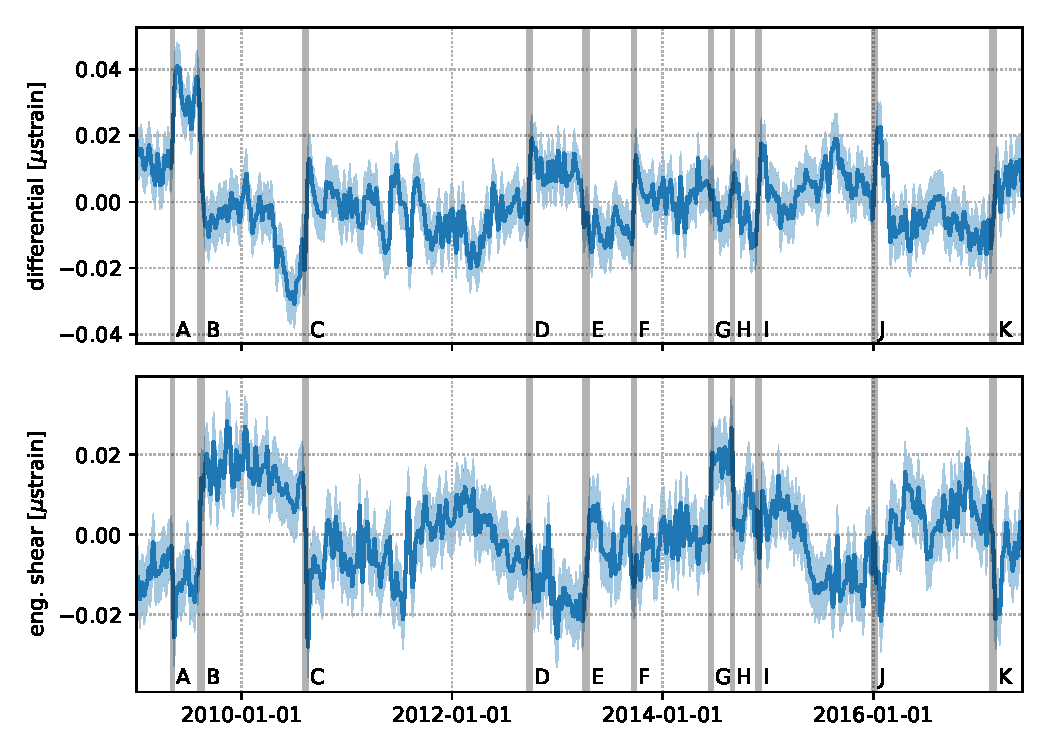
\includegraphics{ch6/figures/gnss.pdf}
\caption
[GNSS derived strains for station B018]
{GNSS derived differential and engineering shear strains for
station B018. The shaded blue regions indicate the one standard
deviation confidence interval. The shaded gray regions indicate times
of strain drops, which are the result of SSEs.}
\label{ch6:fig:Gnss}
\end{figure}

\begin{figure}
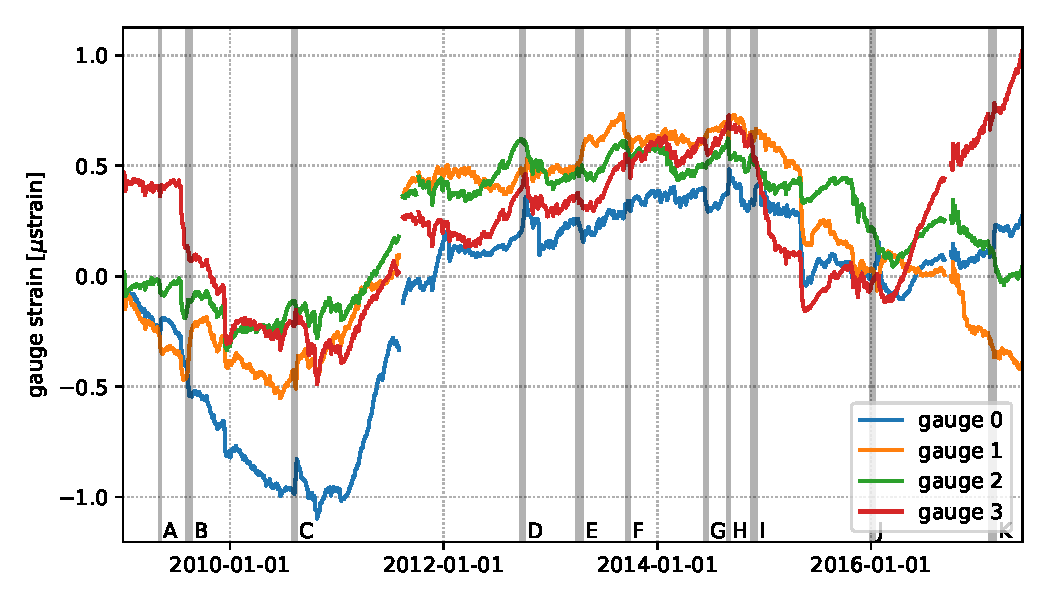
\includegraphics{ch6/figures/gauge.pdf}
\caption
[Gauge readings at station B018]
{Gauge readings at station B018. The gray shaded regions
indicate times of strain drops from Figure \ref{ch6:fig:Gnss}.}
\label{ch6:fig:Gauge}
\end{figure}

\begin{figure}
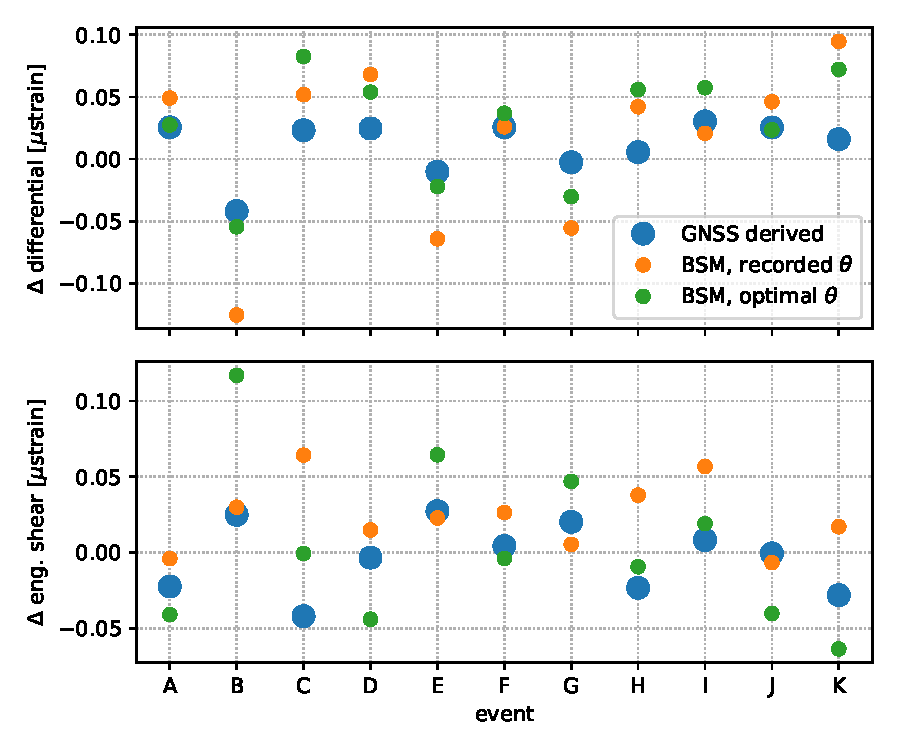
\includegraphics{ch6/figures/fit.pdf}
\caption
[GNSS and BSM strain dropts at station B018]
{GNSS derived strain drops at station B018 during the 11
events identified in Figure \ref{ch6:fig:Gnss} (blue dots), BSM strain
drops using the recorded orientation for B018 (orange dots), and BSM
strain drops using the optimal orientation for B018 (green dots).}
\label{ch6:fig:Fit}
\end{figure}

\begin{figure}
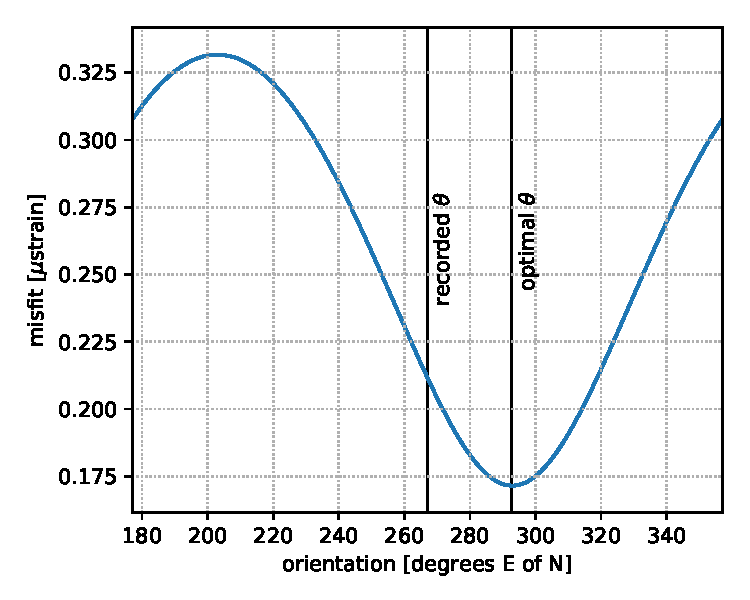
\includegraphics{ch6/figures/misfit.pdf}
\caption
[Misfit as a function of instrument orientation for station
B018]
{Misfit as a function of instrument orientation for station
B018.}
\label{ch6:fig:Misfit}
\end{figure}

The differential and engineering shear strains recorded at station
B018 have notably less noise than most BSMs. Nonetheless, the
engineering shear strains at B018 are not consistent with the GNSS
derived strains. For example, BSM data shows a strain increase from
the summer 2010 SSE, and the GNSS derived strains predict a strain
decrease with about equal magnitude. We consider the possibility that
this discrepancy is due to an error in the instrument orientation, and
we identify a new, optimal orientation for station B018. We want to
find the value for $\theta_0$ that causes the strain drops (or
increases) recorded at B018 to best match the strain drops derived
from GNSS data. We identify 11 strain drops in the GNSS derived
strains, which are due to SSEs in the Puget Sound region and in Oregon
(Figure \ref{ch6:fig:Gnss}). We define strain drops as the total strain
change over the hand-selected intervals shown in Figure
\ref{ch6:fig:Gnss}. The strain drops for each event are shown in Figure
\ref{ch6:fig:Fit}. For each tested $\theta_0$, we use eq.
(\ref{ch6:eq:GaugeToStrain}) to convert the strain drops recorded at each
gauge (Figure \ref{ch6:fig:Gauge}) to the differential and engineering
shear strain drops. We then use the L2 norm of the residuals, the
difference between the BSM strain drops and the GNSS derived strain
drops, as the misfit metric. We find an optimal value of $\theta_0$ to
be $293^\circ$ east of north, which can be compared to the recorded
value of $267^\circ$ (Figure \ref{ch6:fig:Misfit}). With the new
orientation, the engineering shear strain recorded at B018 decreases
during the summer 2010 SSE, which is now consistent with the GNSS data
(Figure \ref{ch6:fig:SSE1}). The differential strains at B018 are roughly
consistent with the GNSS derived strains, regardless of whether the
recorded $\theta_0$ or optimal $\theta_0$ is used.

\section{Conclusion}
We have compared BSM data to GNSS derived strains for eight of the
past SSEs in the Puget Sound region. The summer 2010 SSE produced the
clearest signal in both the BSM data and GNSS derived strain, and yet
it is still difficult to reconcile the two datasets. Of the five BSM
stations that record strain from SSEs, only one of them, B004, records
differential and engineering shear strains that are consistently in
agreement with the GNSS derived strains. For station B003, only the
engineering shear strains are consistent with the GNSS data. Both the
differential and engineering shear strains recorded at B018 can be
made to agree with the GNSS data when assuming a new instrument
orientation. For station B005 and B007 it may be necessary to use a
coupling matrix other than the isotropic one considered in this study.
We are unaware of a reliable calibration method for these stations,
since tidal calibration is not possible. In general, we urge caution
when attempting to use BSM data to describe regional strains.

\begin{figure}
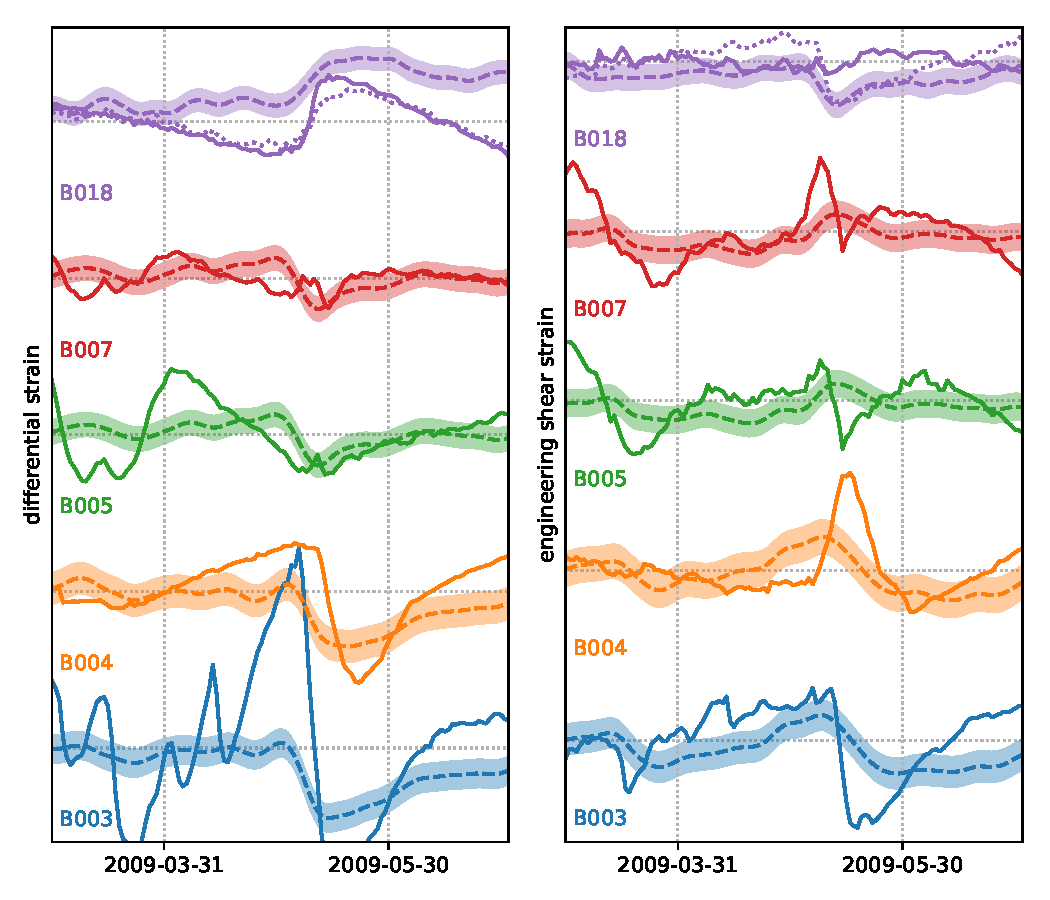
\includegraphics{ch6/figures/SSE0.pdf}
\caption
[BSM and GNSS derived strains for the spring 2009 SSE]
{Same as Figure \ref{ch6:fig:SSE1}, but for the spring 2009 SSE.}   
\label{ch6:fig:SSE0}
\end{figure}

\begin{figure}
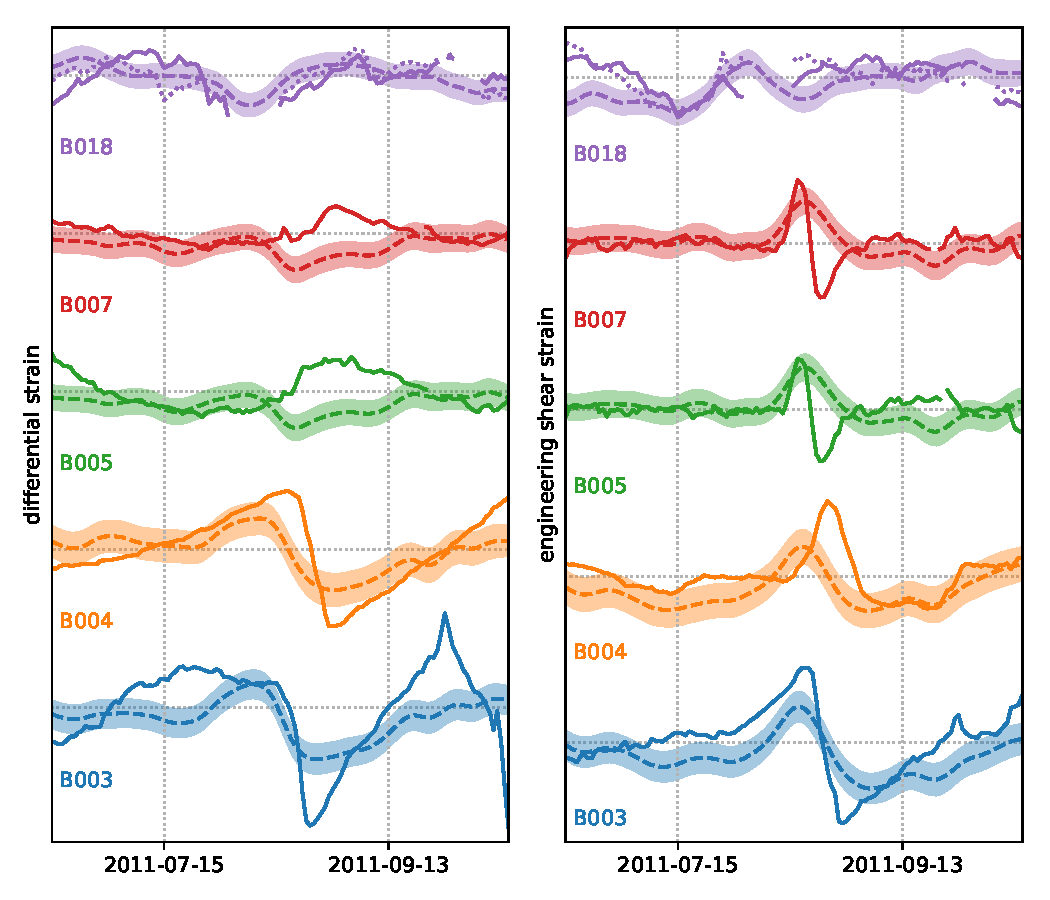
\includegraphics{ch6/figures/SSE2.pdf}
\caption
[BSM and GNSS derived strains for the summer 2011 SSE]
{Same as Figure \ref{ch6:fig:SSE1}, but for the summer 2011 SSE.}   
\label{ch6:fig:SSE2}
\end{figure}

\begin{figure}
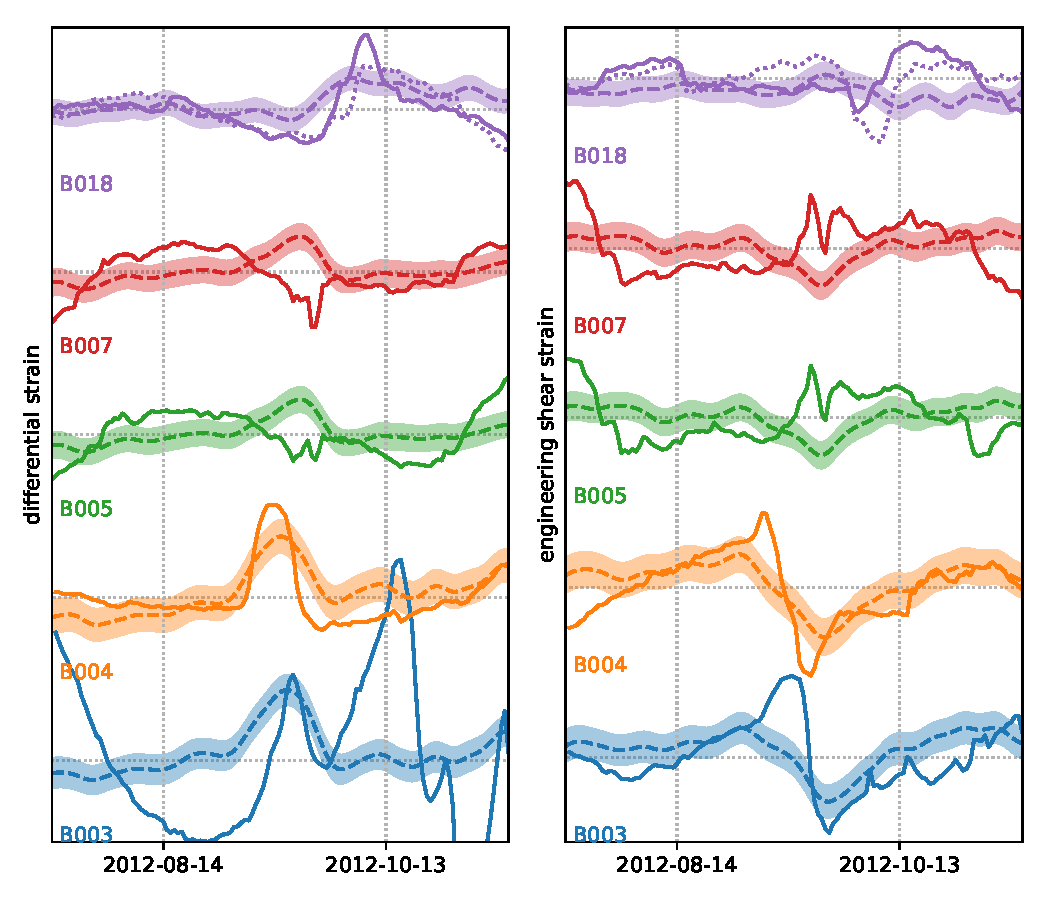
\includegraphics{ch6/figures/SSE3.pdf}
\caption
[BSM and GNSS derived strains for the summer 2012 SSE]
{Same as Figure \ref{ch6:fig:SSE1}, but for the summer 2012 SSE.}   
\label{ch6:fig:SSE3}
\end{figure}

\begin{figure}
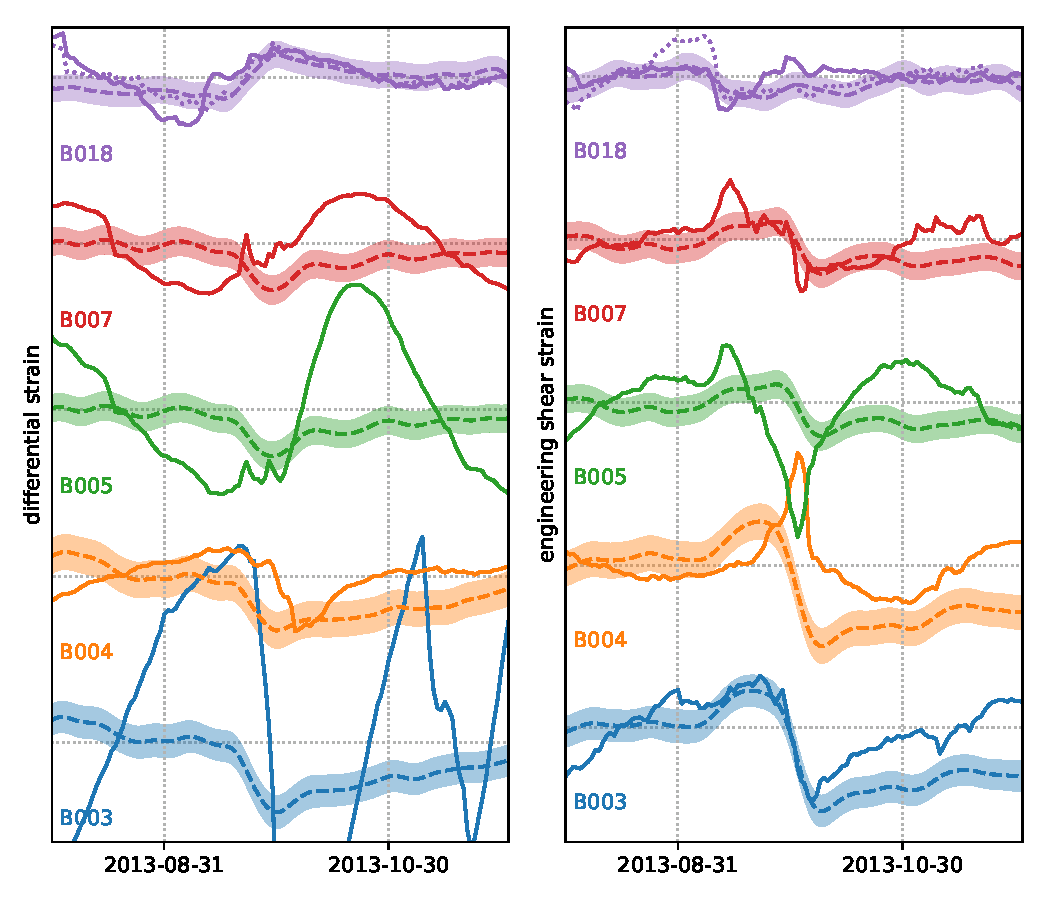
\includegraphics{ch6/figures/SSE4.pdf}
\caption
[BSM and GNSS derived strains for the fall 2013 SSE]
{Same as Figure \ref{ch6:fig:SSE1}, but for the fall 2013 SSE.}   
\label{ch6:fig:SSE4}
\end{figure}

\begin{figure}
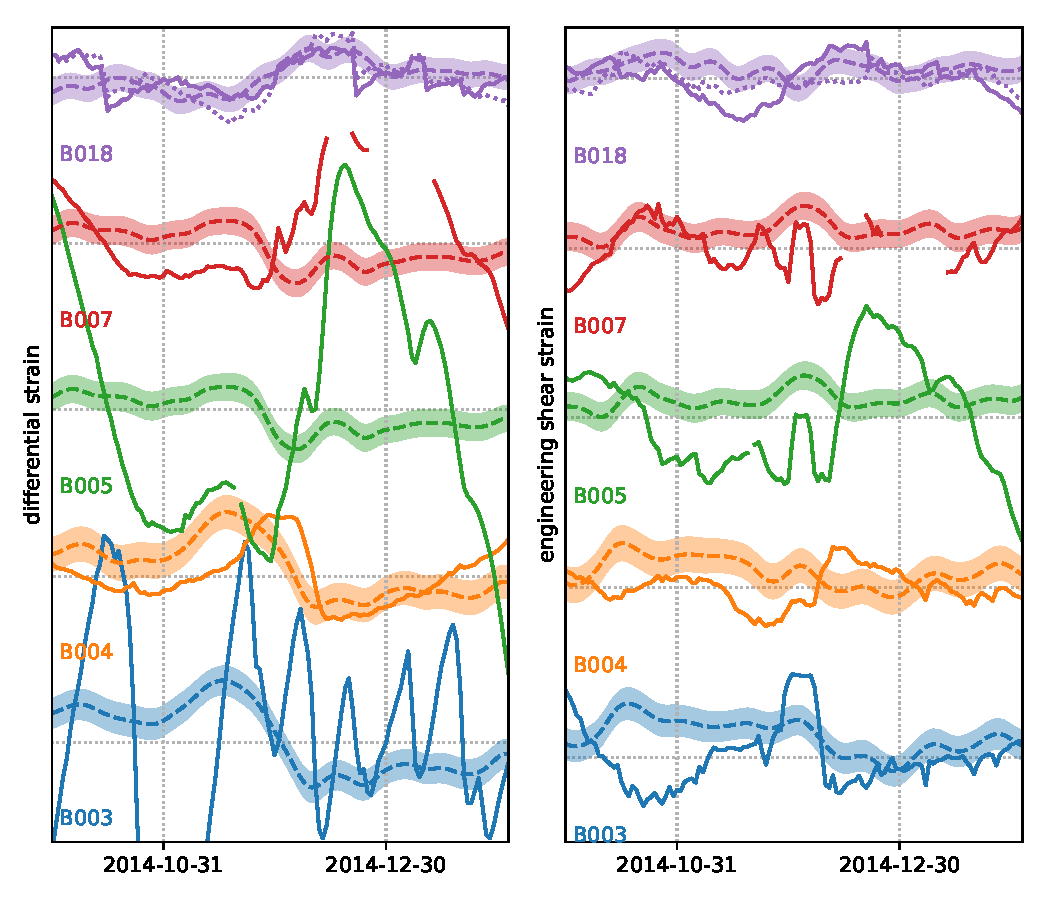
\includegraphics{ch6/figures/SSE5.pdf}
\caption
[BSM and GNSS derived strains for the fall 2014 SSE]
{Same as Figure \ref{ch6:fig:SSE1}, but for the fall 2014 SSE.}   
\label{ch6:fig:SSE5}
\end{figure}

\begin{figure}
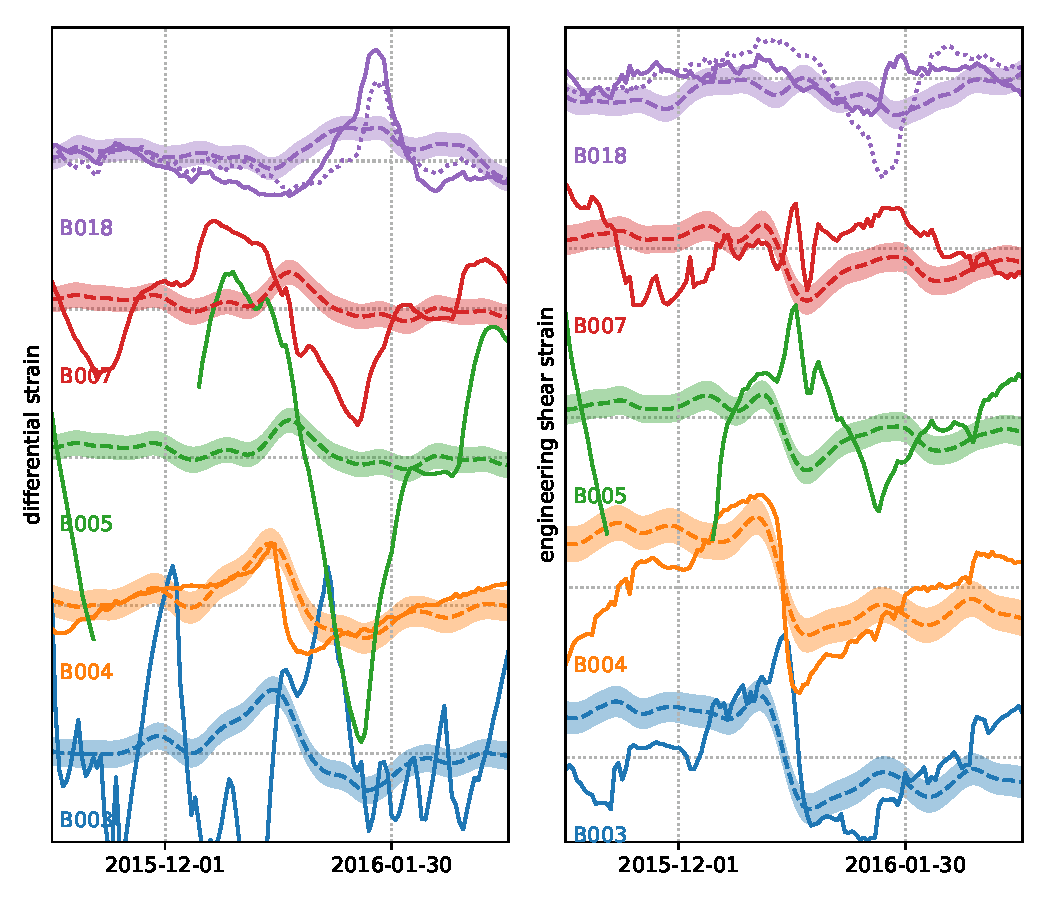
\includegraphics{ch6/figures/SSE6.pdf}
\caption
[BSM and GNSS derived strains for the winter 2015-2016 SSE]
{Same as Figure \ref{ch6:fig:SSE1}, but for the winter 2015-2016 SSE.}   
\label{ch6:fig:SSE6}
\end{figure}

\begin{figure}
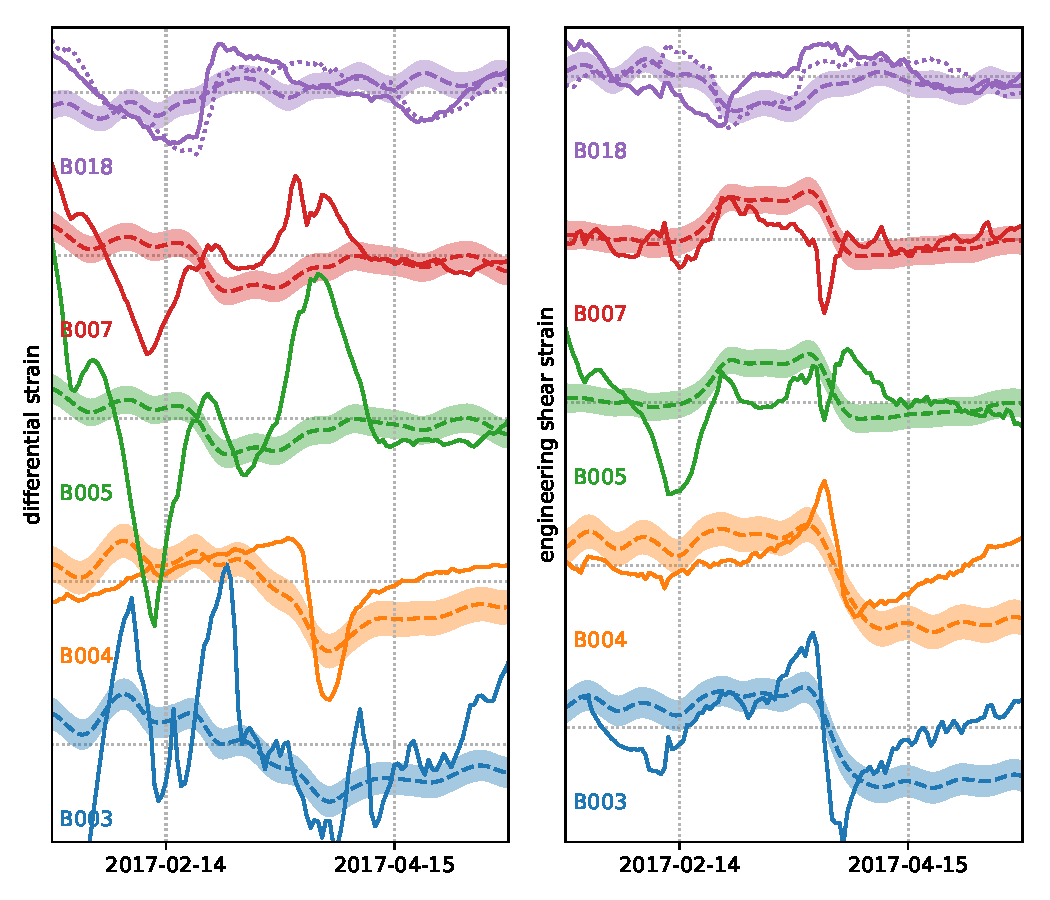
\includegraphics{ch6/figures/SSE7.pdf}
\caption
[BSM and GNSS derived strains for the winter 2017 SSE]
{Same as Figure \ref{ch6:fig:SSE1}, but for the winter 2017 SSE.}   
\label{ch6:fig:SSE7}
\end{figure}

%\bibliographystyle{agu04}
%\bibliography{refs}  
